\section{Portfolio Layout Optimization}

% \subsubsection*{1}
% For each portfolio size $n$, I solved the max-min layout problem
% \[
%     p^\star = \max_{\{s_i\}} \min_{i<j} \|s_i - s_j\|_2
% \]
% over the feasible annular region, while enforcing the two exclusion-zone
% constraints. The implementation first builds deterministic greedy starts from a
% dense set of feasible candidate points on the annulus, exclusion boundaries, and
% interior of the feasible region. Each greedy start repeatedly adds the candidate
% point whose nearest selected neighbor is as far away as possible. The best greedy
% layouts are then used as initial means for CMA-ES, which searches continuously
% over the stock coordinates. Finally, each CMA-ES restart is refined with SLSQP by
% introducing an auxiliary variable $p$ and enforcing all pairwise constraints
% \[
%     \|s_i - s_j\|_2 \ge p.
% \]
% The reported value is the largest feasible minimum pairwise distance found.

\subsubsection*{2}
\begin{verbatim}
2,8.00000000
3,6.92820323
4,5.65685425
5,4.70228202
6,4.00000000
7,3.34926665
8,3.05529777
9,2.74391668
10,2.69575702
\end{verbatim}

\subsubsection*{3}

% For each portfolio size $n \in \{2,\ldots,10\}$, the stock locations were chosen to maximize the minimum pairwise Euclidean distance
% \[
%     p^\star = \max_{\{s_i\}} \min_{i<j} \|s_i - s_j\|_2,
% \]
% subject to the annular feasible region and the two exclusion-zone constraints. The theoretical diversification efficiency was then computed as
% \[
%     \eta = \frac{1}{1 + 1/p^\star}.
% \]

\begin{figure}[H]
    \centering
    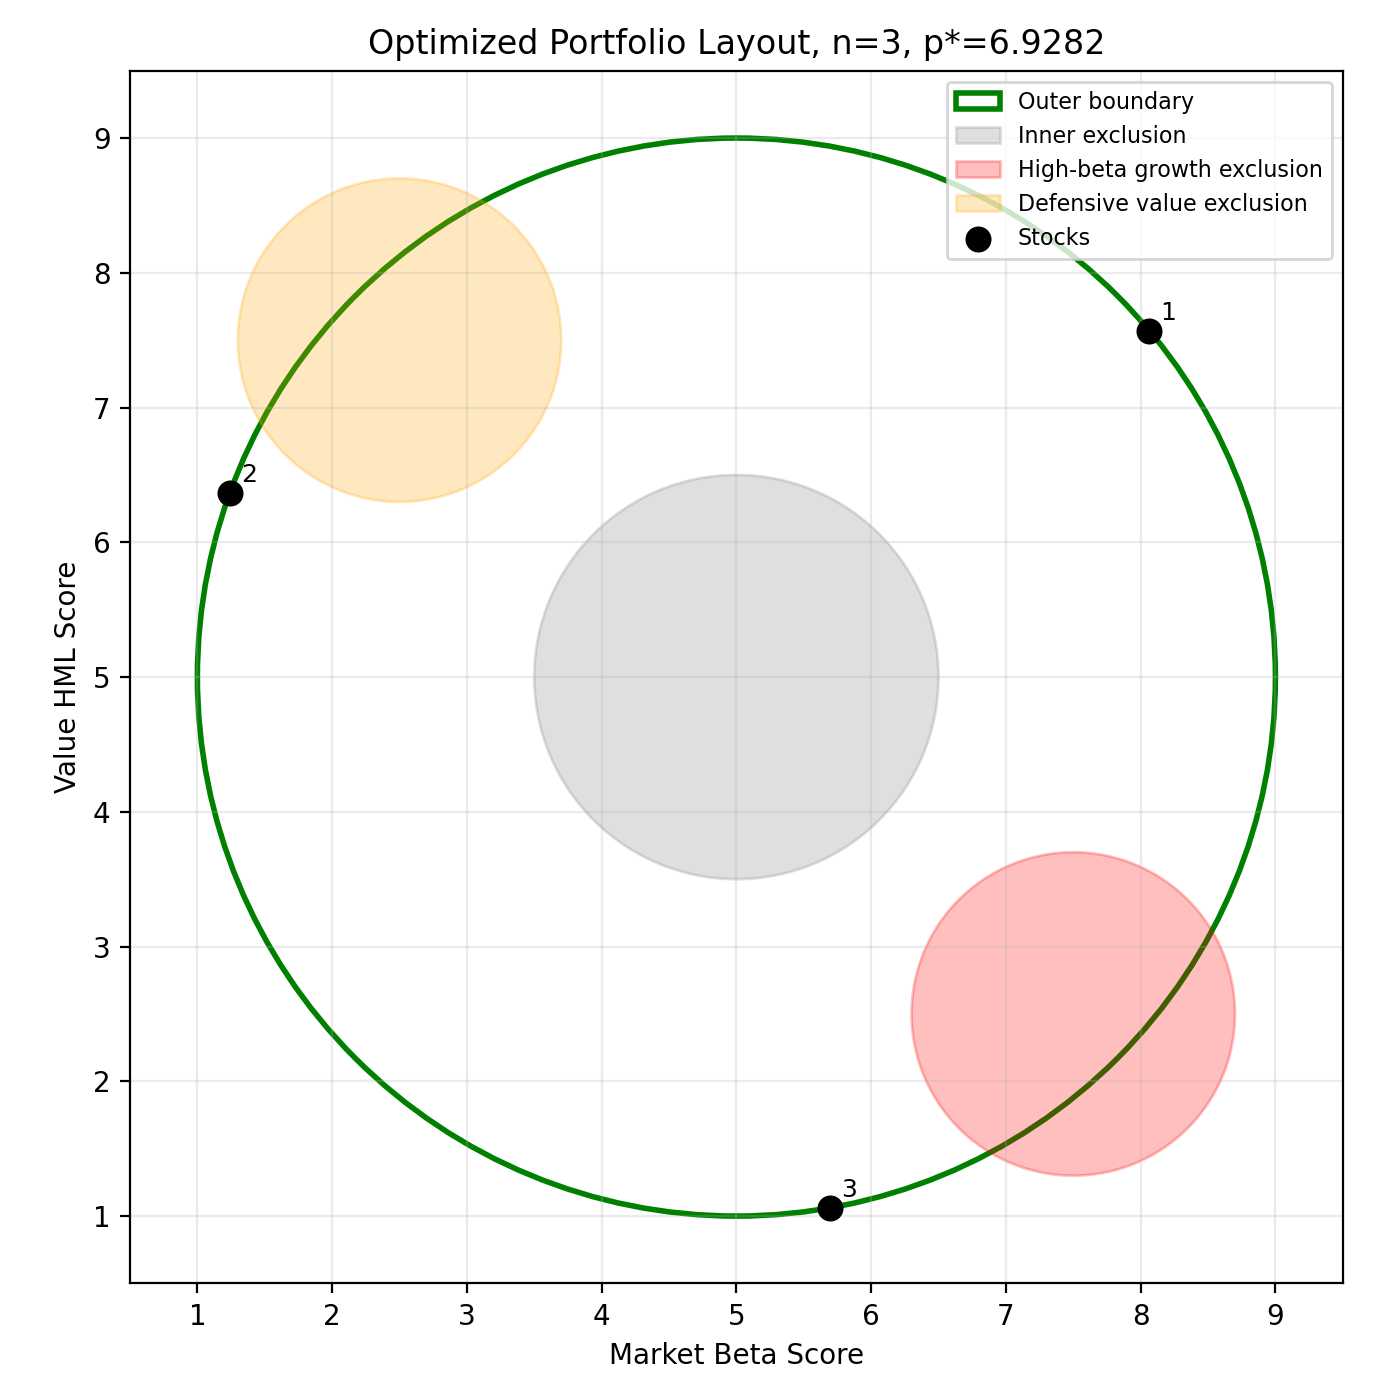
\includegraphics[width=0.6\linewidth]{img/layout_n3.png}
    \caption{(a) $n=3$}
    % \caption{Optimized stock layouts with constraint boundaries.}
\end{figure}
\begin{figure}[H]
    \centering
    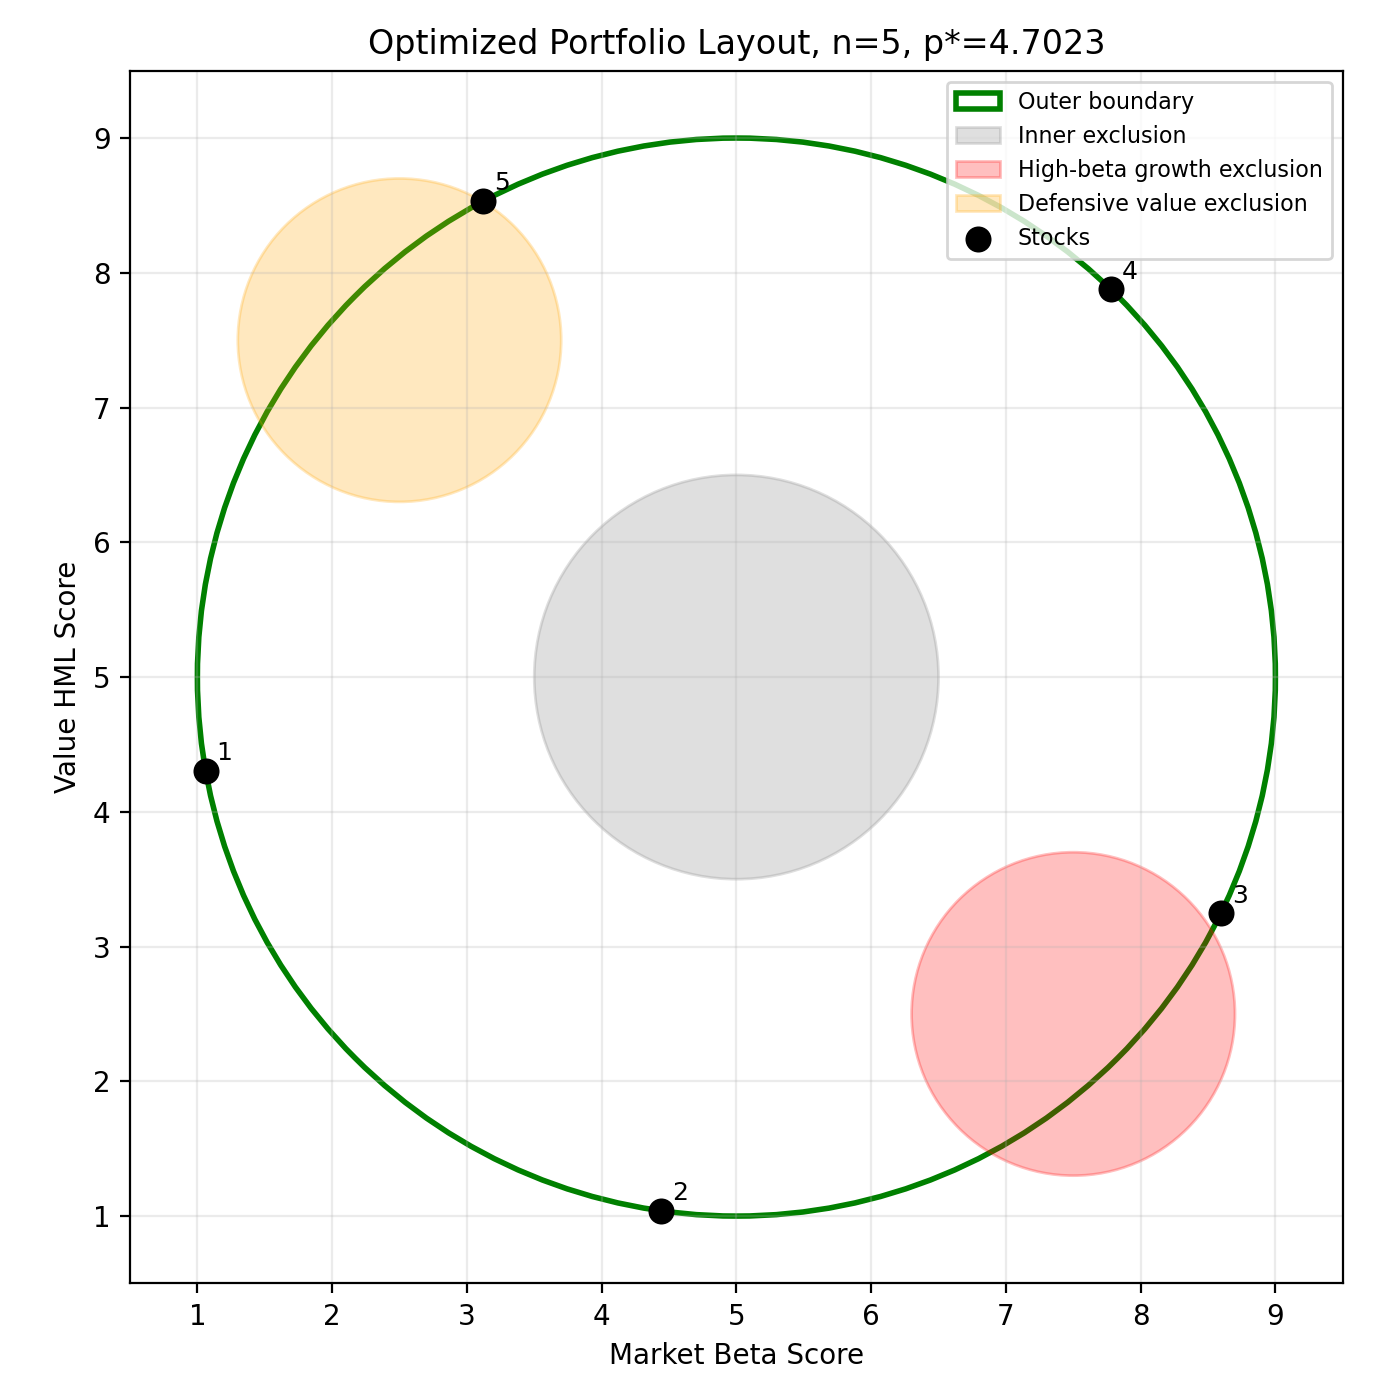
\includegraphics[width=0.6\linewidth]{img/layout_n5.png}
    \caption{(b) $n=5$}
\end{figure}
\begin{figure}[H]
    \centering
    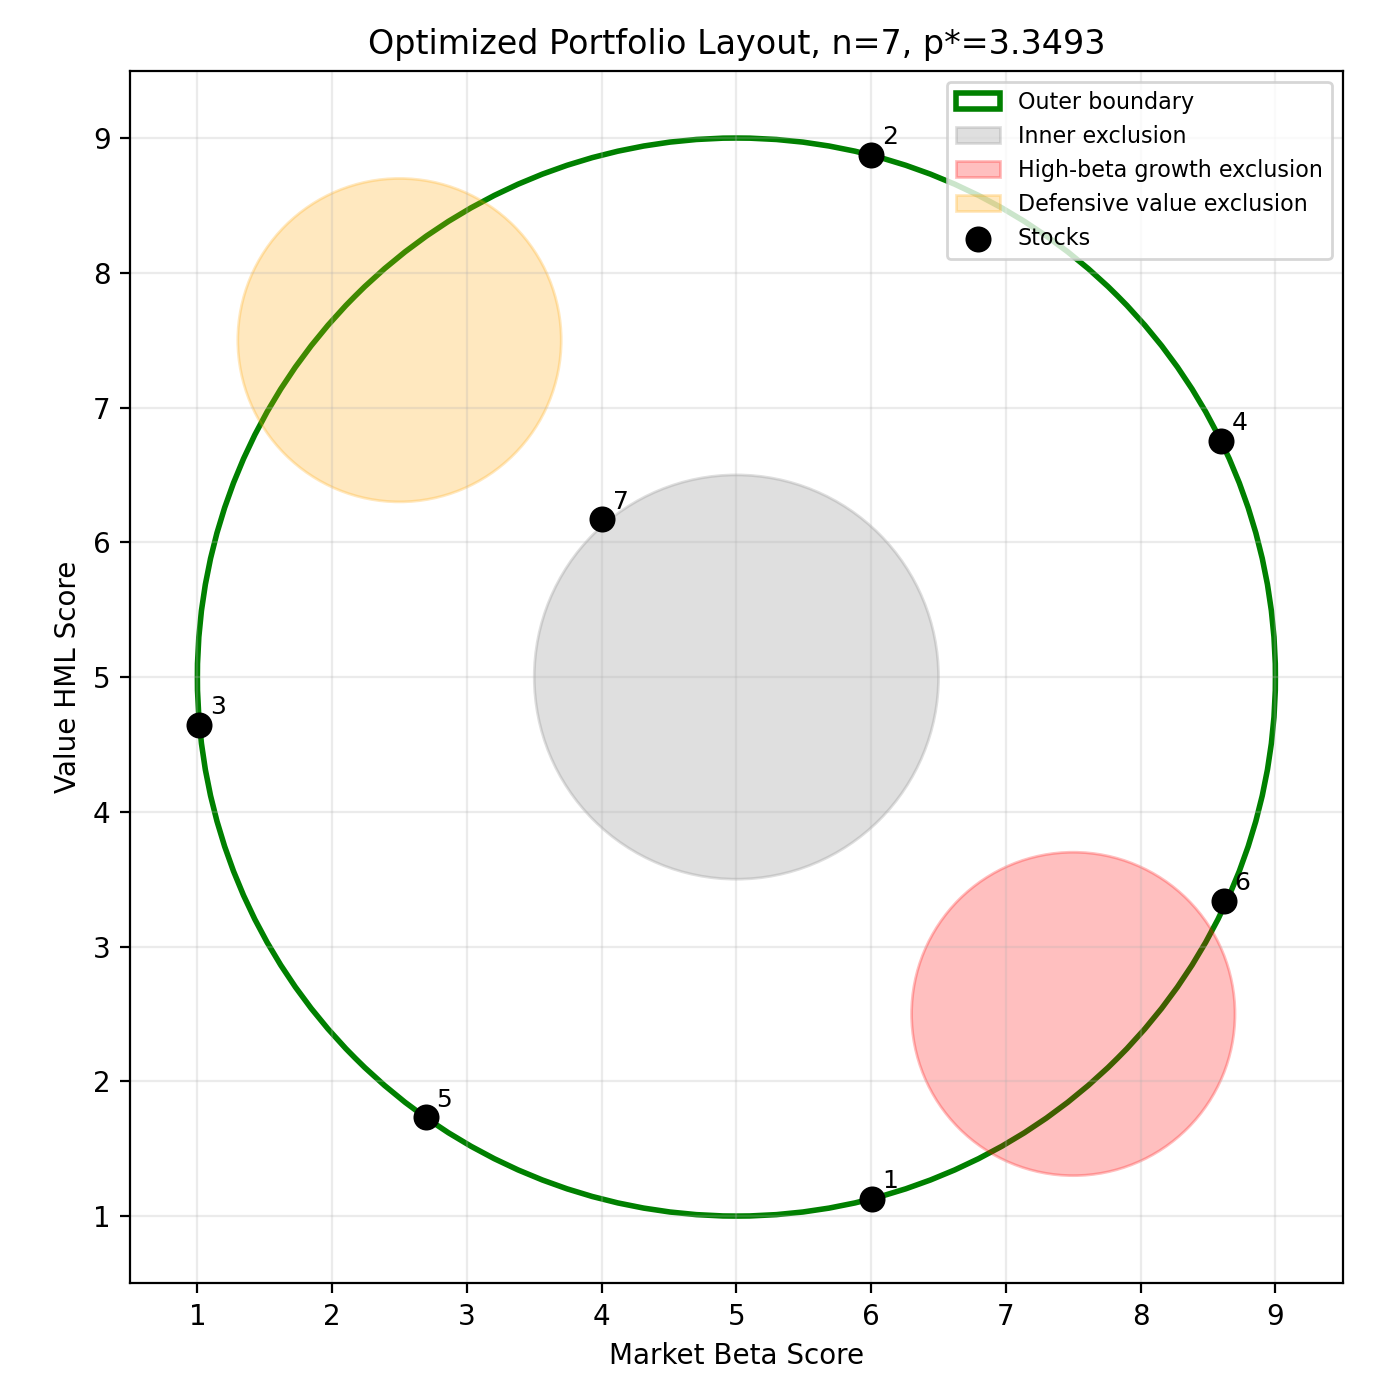
\includegraphics[width=0.6\linewidth]{img/layout_n7.png}
    \caption{(c) $n=7$}
\end{figure}

\subsubsection*{4}
\begin{figure}[H]
    \centering
    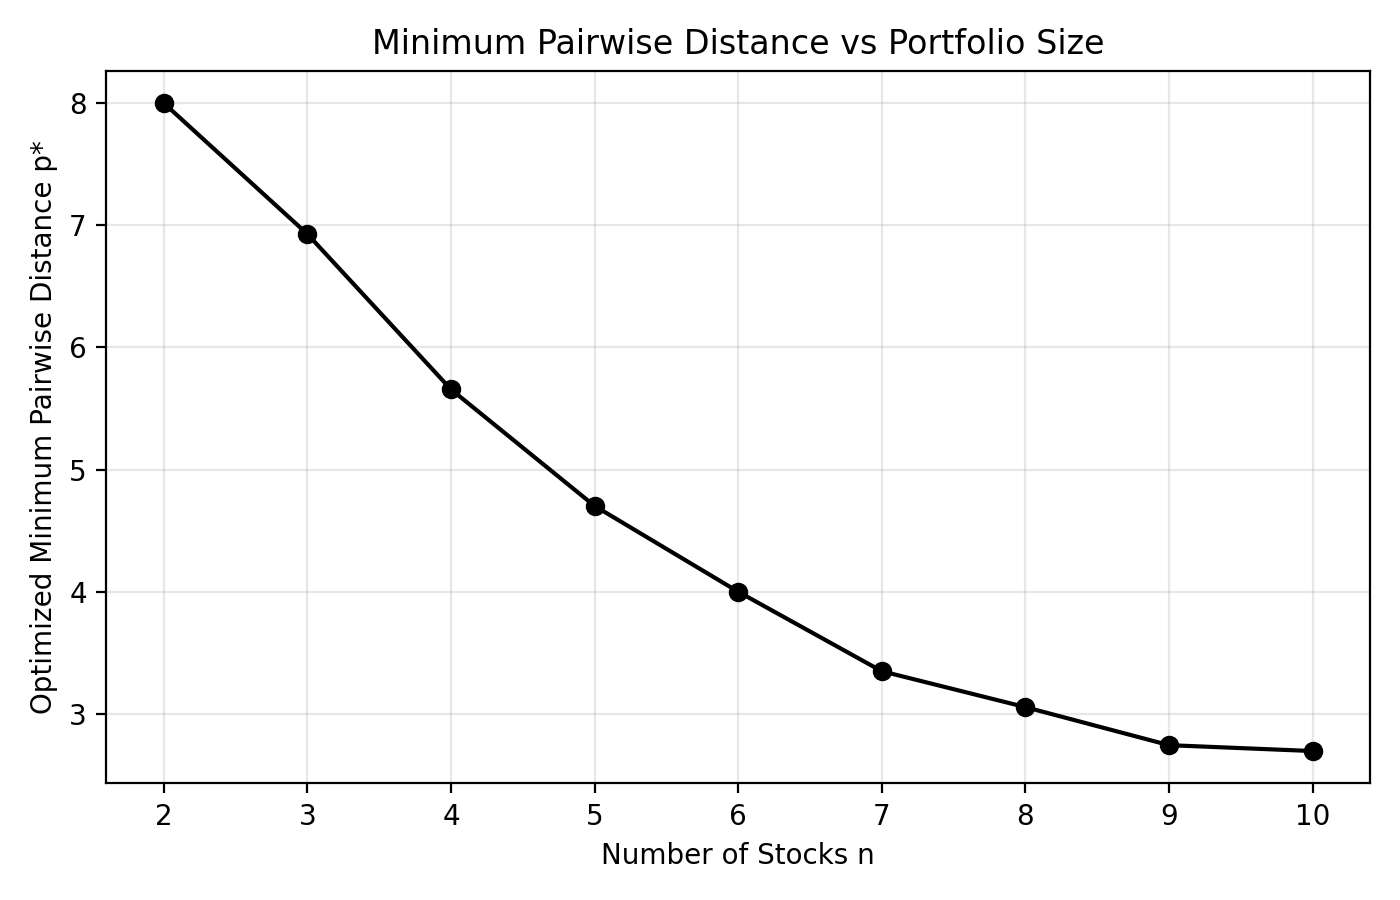
\includegraphics[width=0.82\linewidth]{img/minimum_distance_vs_n.png}
    \caption{Minimum pairwise distance $p^\star$ versus number of stocks.}
\end{figure}

\subsubsection*{5}
\begin{figure}[H]
    \centering
    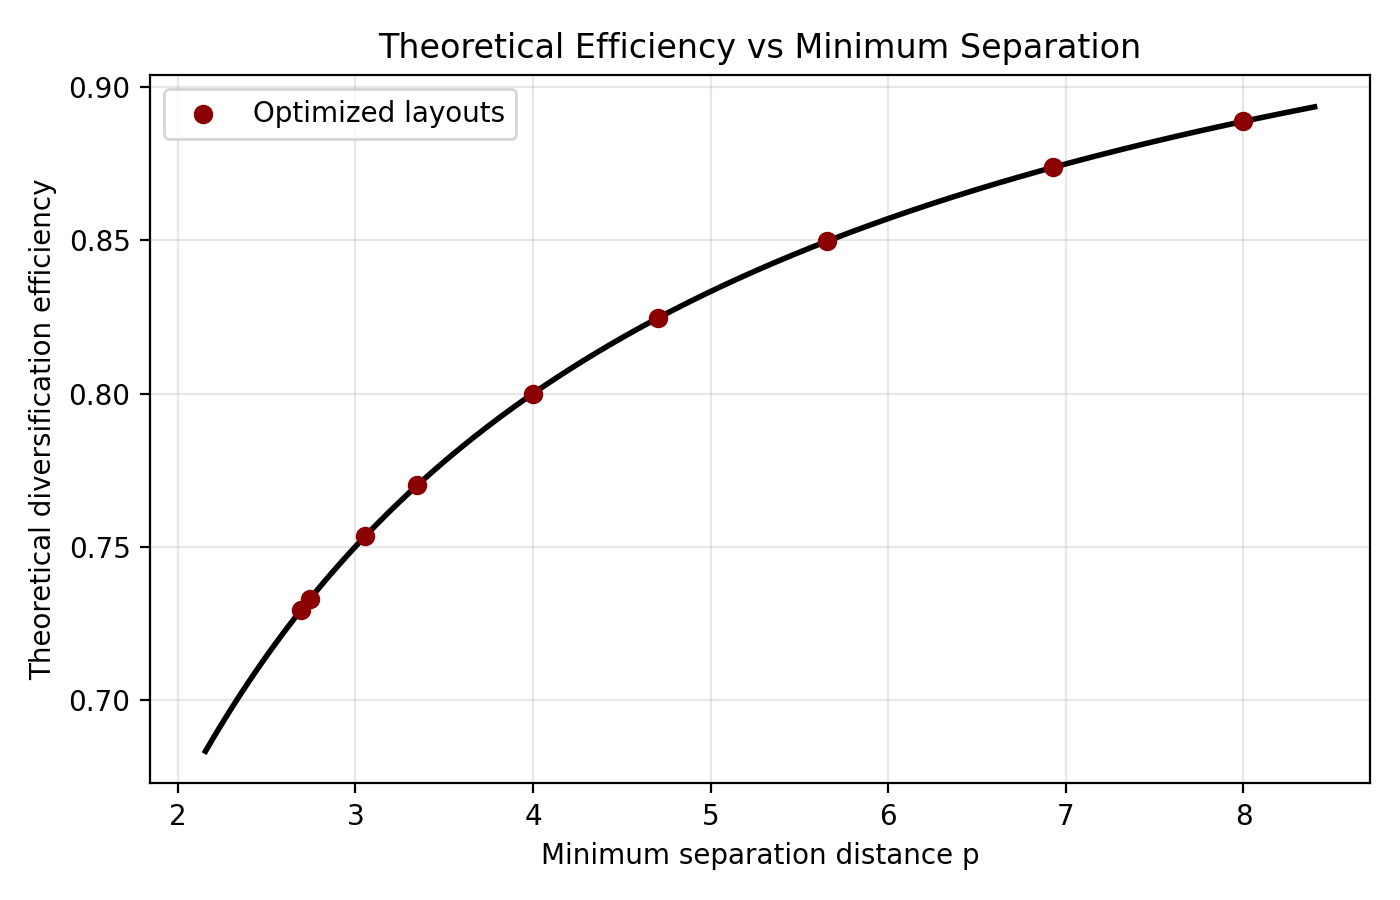
\includegraphics[width=0.82\linewidth]{img/theoretical_efficiency_vs_distance.png}
    \caption{Theoretical diversification efficiency as a function of $p^\star$}
\end{figure}

\subsection*{Code}
The implementation is included in \hyperref[gp_efficiency]{Appendix~\ref*{portfolio_layout_opt}}.
